% Generated from arXiv:2605.03277; see tools/build_source_compendium.py.
\section{Calculation laboratory VIII-B: Two-horizon spectra and continuum response}
\label{lab:2605_03277}

\calculationroute
  {Two-horizon boundary conditions, black-hole complex scaling, continuum level density, and coupled-channel diagonalization.}
  {Two-horizon complex scaling, QNM and continuum-level-density data, greybody response, coupled string-inspired channels, higher dimensions, and block-balancing diagnostics.}
  {Compute two-horizon QNMs and continuum response, then diagnose coupled-channel and block-balancing effects.}

This Laboratory reconstructs the calculation underlying
Ref.~\cite{Ogawa:2026dSCSM}.  Two-horizon boundary conditions, the Gaussian
basis, and continuum level density have already been derived.  The worked
calculation therefore opens with the parameter scan and retains the numerical
response, coupled-channel, higher-dimensional, and conditioning analyses.

\begin{comment}
\subsection{Setup}\label{src:2605_03277:sec:setup}
\subsubsection{Complex scaling and non-Hermitian spectral problem}
\label{src:2605_03277:sec:setup-csm}
The complex scaling method is implemented by rotating the tortoise coordinate
as
\begin{align}
    r_* \mapsto r_* \rme^{\rmi\theta},
\end{align}
with a real scaling angle $\theta$.
Under this transformation, the original outgoing-wave boundary-value problem
is converted into a non-Hermitian spectral problem for the complex-scaled
operator,
\begin{align}
    H^\theta \psi_l^\theta = \omega^2 \psi_l^\theta .
\end{align}
The essential point is that resonance poles, which are defined through
outgoing boundary conditions in the original problem, appear as discrete
eigenvalues of $H^\theta$ after complex scaling.
Note that $\omega$ for any resonance state does not depend on~$\theta$.
This provides a common spectral framework in which pole and continuum sectors
may be discussed simultaneously.
\subsubsection{Basis expansion and generalized eigenvalue problem}
\label{src:2605_03277:sec:setup-basis}
To solve the complex-scaled problem numerically, we expand the wave function
in a finite set of $L^2$~basis functions,
\begin{align}
    \psi^\theta(r_*)
    =
    \sum_i c_i \phi_i(r_*).
\end{align}
The explicit choice of basis functions has been considered in the numerical
analysis of Ref.~\cite{Ogawa:2026veu}, and it may be natural to choose the Polynomial $\times$ real range Gaussian basis
\begin{align}
    \phi_{i,n}(r_*)
    \propto
    (\sqrt{\alpha_i}\, r_*)^n \rme^{-\alpha_i r_*^2},
    \qquad
    \text{$n=0$, $1$, $2$, \dots, $p_{\max}$} .
\end{align}
Here, $\alpha_i = 1/r_i^2$, and
the Gaussian ranges in $[r_{*0},r_{*\max}]$ are taken in geometric progression,
\begin{align}
    r_i = r_{*0}\, a^{\,i-1},
    \qquad
    a = \left( \frac{r_{*\max}}{r_{*0}} \right)^{1/(i_{\max}-1)},
    \label{src:2605_03277:eq:gaussian-ranges}
\end{align}
With this expansion, the complex-scaled equation is reduced to a matrix
eigenvalue problem of the form
\begin{align}
    \sum_j
    \left(
        H^\theta_{ij}
        -\omega^2 N_{ij}
    \right)c_j
    =0,
\end{align}
where $H^\theta_{ij}$ and $N_{ij}$ denote the Hamiltonian and overlap matrices,
respectively.
The resulting eigenvalues provide the basic spectral data used in the
subsequent QNM and CLD analyses.
\subsubsection{Continuum level density}
\label{src:2605_03277:sec:setup-cld}
Besides the isolated resonance poles identified with QNM frequencies, the
complex-scaled spectrum also contains information on the continuum sector.
A useful quantity for this purpose is the continuum level density (CLD), which
measures how the continuum is modified by the interaction relative to a
reference problem.
Let $H$ be the Hamiltonian of the black-hole perturbation problem and let
$H_0$ be a suitable reference (non-interacting) Hamiltonian.
In the present work, the most natural choice is the asymptotic free operator,
so that the CLD describes the deformation of the continuum induced by the
black-hole potential.
The CLD is defined by
\begin{align}
    \Delta \rho(E)
    =
    -\frac{1}{\pi}
    \im
    \Tr
    \left[
        \frac{1}{E-H+\rmi 0}
        -
        \frac{1}{E-H_0+\rmi 0}
    \right],
\end{align}
where $E$ denotes the spectral parameter \cite{Suzuki:2005wv,Avishai:1985,Myo:2014ypa}.
In the present Schr\"odinger-type problem, we identify
\begin{align}
    E=\omega^2 .
\end{align}
After complex scaling, one may equivalently evaluate the CLD from the
complex-scaled operators,
\begin{align}
    \Delta \rho^\theta(E)
    =
    -\frac{1}{\pi}
    \im
    \Tr
    \left[
        \frac{1}{E-H^\theta}
        -
        \frac{1}{E-H_0^\theta}
    \right],
    \label{src:2605_03277:eq:cld_csm}
\end{align}
where $H^\theta$ and $H_0^\theta$ denote the complex-scaled Hamiltonians.
In an exact treatment, the resulting CLD is independent of the scaling angle
within the admissible range, while in a finite-basis calculation a residual
$\theta$ dependence remains and may be used as a practical measure of
numerical stability.
From the physical point of view, the CLD complements the QNM frequencies by
probing the continuum response.
In asymptotically flat black holes, this sector is closely related to
branch-cut contributions and late-time tails.
In the present work, we use the CLD as a diagnostic of how the continuum
sector is reorganized in dS$_4$ backgrounds within the same CSM
framework that yields the QNM poles.
For this reason, we leave the construction of an appropriate reference
Hamiltonian $H_0$ for the AdS case, compatible with the AdS boundary
condition, as an interesting and highly subtle problem for future work.
\end{comment}
\subsection{QNM and CLD for dS black holes}\label{src:2605_03277:sec:result}
\subsubsection{Numerical results of QNMs}
We first present the QNM frequencies obtained by applying the present CSM
framework to four-dimensional Schwarzschild--dS black holes.
The purpose of this subsection is twofold.
First, we check that the complex-scaled formulation can identify isolated
resonance eigenvalues also in the presence of a nonzero cosmological constant.
Second, we examine how the low-lying QNM spectrum changes as the cosmological
constant $\Lambda$ is varied.
We consider scalar, electromagnetic, and gravitational perturbations,
corresponding to $s=0$, $s=1$, and $s=2$, respectively.
For each spin sector, we compute two representative angular momenta,
which we denote by $l=2$ and $l=3$.
The notation $l$ is used throughout this paper for the angular momentum
quantum number.
For each value of $\Lambda$, the corresponding Schwarzschild--dS
Regge--Wheeler-type potential is inserted into the complex-scaled
Schr\"odinger equation, and the QNM candidates are extracted as isolated
eigenvalues separated from the rotated continuum.
The identification of QNM candidates is performed by looking for isolated
eigenvalues that remain stable under changes of the numerical parameters.
In the numerical analysis below, we focus on the low-lying modes.
As in the Schwarzschild and Reissner--Nordstr\"om analysis of our previous
work, these modes are expected to be the most stable against changes of the
basis size, basis parameters, integration range, and scaling angle.
By contrast, higher overtones are typically broader and lie closer to the
rotated continuum, making their identification more sensitive to numerical
details.
For this reason, the present calculation should be understood as a first
systematic test of the CSM framework for Schwarzschild--dS backgrounds,
rather than as a final optimized computation of all overtones.
For each channel, we perform calculations for several values of the
cosmological constant.
Positive values,
\begin{align}
    \Lambda>0,
\end{align}
correspond to Schwarzschild--dS backgrounds.
The limit $\Lambda\to0$ connects the present setup to the asymptotically flat
Schwarzschild problem and therefore serves as an important reference point.
Particular attention will be paid to how the real and imaginary parts of the
QNM frequencies move as $\Lambda$ is varied.
The numerical results are summarized in
Figs.~\ref{src:2605_03277:fig:qnm_ds_s0}--\ref{src:2605_03277:fig:qnm_ds_s2}
for Schwarzschild--dS.
Here
Fig.~\ref{src:2605_03277:fig:qnm_ds_s0} shows the scalar results,
Fig.~\ref{src:2605_03277:fig:qnm_ds_s1} shows the electromagnetic results, and
Fig.~\ref{src:2605_03277:fig:qnm_ds_s2} shows the gravitational results.
In these figures, we fix the magnitude of the cosmological constant to
$\Lambda=0.08$.
For each channel, we combine the results obtained for several values of the
scaling angle,
\begin{align}
    \theta = 42^\circ\text{--}44^\circ ,
\end{align}
and for the Gaussian parameter sets
\begin{align}
    i_{\max}=30,\ 40,
    \qquad
    r_{*0}=0.1,
    \qquad
    r_{*\max}=60,\ 80 .
\end{align}
The complex eigenvalues of the complex-scaled Hamiltonian are displayed in the
complex $\omega$ plane.
The QNM candidates are identified as isolated eigenvalues that remain stable
under these moderate changes of the scaling angle and basis parameters.
\begin{figure}[htbp]
 \centering
 \resizebox{\textwidth}{!}{%
 \begin{tikzpicture}
  \node at (0,8) {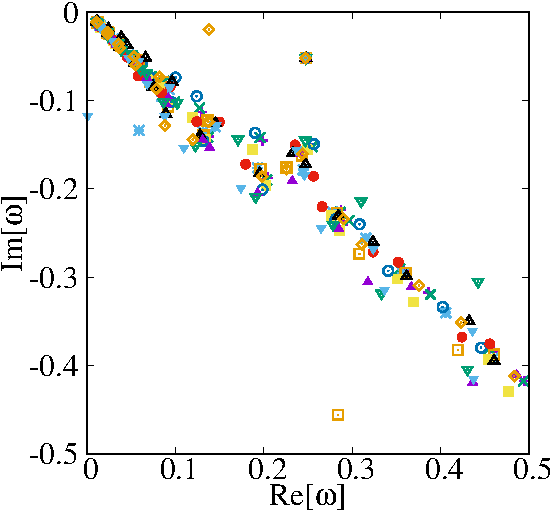
\includegraphics[width=0.45\linewidth]{source_compendium/figures/2605_03277/fig/ene_SdS_s0_l2_lam0.08.pdf}};
  \node at (8,8) {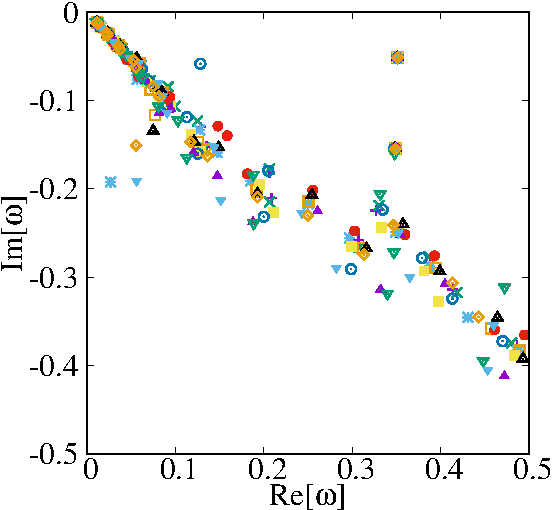
\includegraphics[width=0.45\linewidth]{source_compendium/figures/2605_03277/fig/ene_SdS_s0_l3_lam0.08.pdf}};
  \node[draw, rectangle] at (-1,8) {$l=2$};
  \node[draw, rectangle] at (7,8) {$l=3$};
  \draw[thick, red] (0.425,10.65) circle (0.3);
  \node[above] at (1.2,10.6) {$n=0$};
  %\draw[thick, red] (1.75,8.3) circle (0.3);
  %\node[above] at (1.75,8.6) {$n=1$};
  \draw[thick, red] (9.65,10.65) circle (0.3);
  \node[above] at (10.655,10.7) {$n=0$};
  \draw[thick, red] (9.55,9.45) circle (0.3);
  \node[above] at (10.45,9.2) {$n=1$};
 \end{tikzpicture}
 }
 \caption{The Schwarzschild--dS case with $s=0$. $M=1.0$.
 The discretized continuum spectrum is represented by the sequence of points aligned approximately along the $\theta$-rotated direction.
 The isolated points on the real-axis side are the QNM frequencies.
 Eigenvalues of the complex-scaled Hamiltonian $H^\theta$ for $l=2$ and $l=3$ are shown.
 The scaling angle is taken to be~$\theta=42^\circ$--$44^\circ$.
 In these figures, we fix the cosmological-constant parameter to $\Lambda=0.08$.
 The eigenvalues enclosed by red circles are identified as QNM candidates, since they appear as isolated points separated from the rotated continuum and remain stable under moderate changes of the scaling angle and basis parameters.}
 \label{src:2605_03277:fig:qnm_ds_s0}
\end{figure}
\begin{figure}[htbp]
 \centering
 \resizebox{\textwidth}{!}{%
 \begin{tikzpicture}
  \node at (0,8) {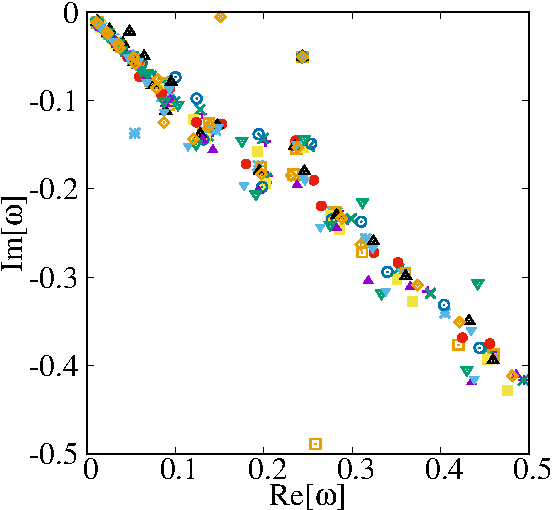
\includegraphics[width=0.45\linewidth]{source_compendium/figures/2605_03277/fig/ene_SdS_s1_l2_lam0.08.pdf}};
  \node at (8,8) {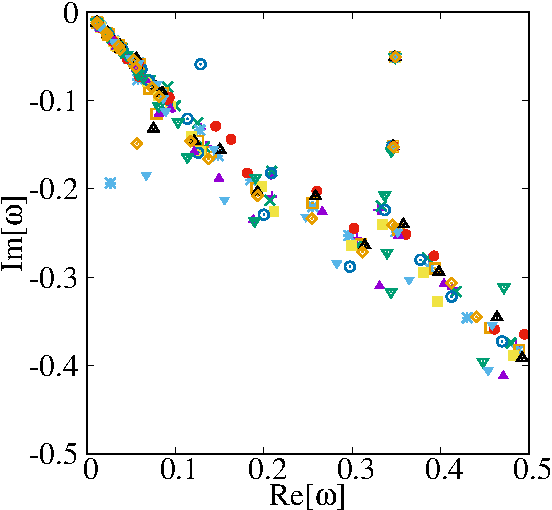
\includegraphics[width=0.45\linewidth]{source_compendium/figures/2605_03277/fig/ene_SdS_s1_l3_lam0.08.pdf}};
  \node[draw, rectangle] at (-1,8) {$l=2$};
  \node[draw, rectangle] at (7,8) {$l=3$};
  \draw[thick, red] (0.4,10.7) circle (0.3);
  \node[above] at (1.625,10.6) {$n=0$};
  %\draw[thick, red] (0.35,9.5) circle (0.3);
  %\node[above] at (1.5,9.5) {$n=1$};
  \draw[thick, red] (9.6,10.65) circle (0.3);
  \node[above] at (10.655,10.7) {$n=0$};
  \draw[thick, red] (9.55,9.45) circle (0.3);
  \node[above] at (10.45,9.2) {$n=1$};
 \end{tikzpicture}
 }
 \caption{The Schwarzschild--dS case with $s=1$. $M=1.0$.}
 \label{src:2605_03277:fig:qnm_ds_s1}
\end{figure}
\begin{figure}[htbp]
 \centering
 \resizebox{\textwidth}{!}{%
 \begin{tikzpicture}
  \node at (0,8) {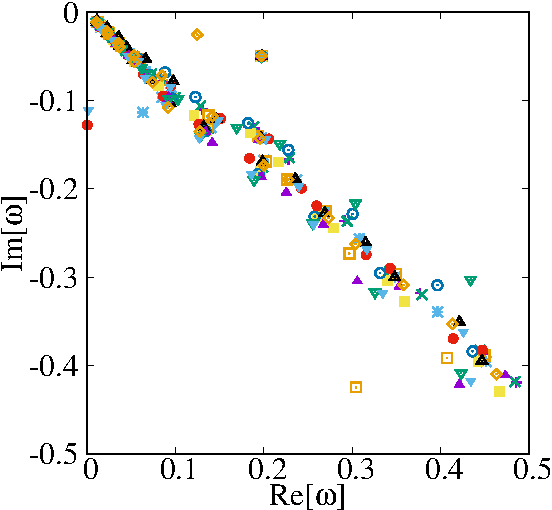
\includegraphics[width=0.45\linewidth]{source_compendium/figures/2605_03277/fig/ene_SdS_s2_l2_lam0.08.pdf}};
  \node at (8,8) {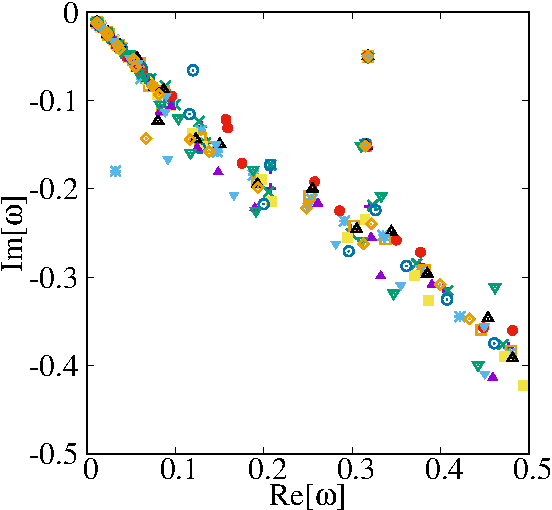
\includegraphics[width=0.45\linewidth]{source_compendium/figures/2605_03277/fig/ene_SdS_s2_l3_lam0.08.pdf}};
  \node[draw, rectangle] at (-1,8) {$l=2$};
  \node[draw, rectangle] at (7,8) {$l=3$};
  \draw[thick, red] (-0.2,10.65) circle (0.3);
  \node[above] at (0.8,10.6) {$n=0$};
  %\draw[thick, red] (1.75,8.3) circle (0.3);
  %\node[above] at (1.75,8.6) {$n=1$};
  \draw[thick, red] (9.25,10.65) circle (0.3);
  \node[above] at (10.2,10.7) {$n=0$};
  \draw[thick, red] (9.2,9.5) circle (0.3);
  \node[above] at (10.1,9.2) {$n=1$};
 \end{tikzpicture}
 }
 \caption{The Schwarzschild--dS case with $s=2$. $M=1.0$.}
 \label{src:2605_03277:fig:qnm_ds_s2}
\end{figure}
The QNM candidates are identified as the eigenvalues enclosed by the red
circles in Figs.~\ref{src:2605_03277:fig:qnm_ds_s0}--\ref{src:2605_03277:fig:qnm_ds_s2}. These eigenvalues
appear as isolated points separated from the rotated continuum and remain
stable under moderate changes of the scaling angle and basis parameters.
We find that the resulting frequencies agree with the previous results of
Ref.~\cite{Zhidenko:2003wq} with high accuracy, which provides a nontrivial validation of
the present CSM identification procedure.
Table~\ref{src:2605_03277:tab:result_ds} presents the numerical
results obtained by the CSM for the Schwarzschild--dS case.
In this table, we list the lowest QNM frequencies, $n=0$, for scalar
($s=0$), electromagnetic ($s=1$), and gravitational ($s=2$) perturbations.
For each spin sector, the results for $l=2$ and $l=3$ are shown for several
values of the cosmological constant~$\Lambda$.
The numbers in parentheses indicate the numerical uncertainty estimated from
the spread of the results obtained with different values of the scaling angle
and basis parameters.
%\footnote{To estimate the numerical uncertainty of the extracted QNM frequencies, we use the spread of the results obtained from different numerical parameter sets. Let $\omega_i$ denote the frequency obtained in the $i$th run, and let $\vsub{N}{samp}$ be the number of runs. We define the averaged frequency by
%\begin{align}
%    \bar{\omega}
%    =
%    \frac{1}{\vsub{N}{samp}}
%    \sum_{i=1}^{\vsub{N}{samp}}
%    \omega_i ,
%\end{align}
%and estimate the numerical uncertainty as $\Delta\omega=\max_i\left|\omega_i-\bar{\omega}\right|$. We then quote the result as $\omega=\Bar{\omega}\pm\Delta\omega$. The quantity $\Delta\omega$ should be understood as a practical measure of numerical stability, not as a statistical error bar.}
\begin{table}[htbp]
\centering
\caption{Numerical results of lowest QNM frequencies ($n=0$) of Schwarzschild--dS black hole for $l=2$ and $l=3$.
The entries are given as
$\omega=\re\omega-\rmi|\im\omega|$.
For comparison, the table also includes the Schwarzschild results obtained
from a separate calculation ($\Lambda=0$).
The numbers in parentheses indicate the numerical uncertainty estimated from
the spread under changes of the scaling angle and basis parameters.}
\label{src:2605_03277:tab:result_ds}
\begin{tabular}{l
                l@{$-\rmi$}l
                l@{$-\rmi$}l}
\toprule
$\Lambda$ & \multicolumn{2}{c}{$l=2$} & \multicolumn{2}{c}{$l=3$} \\
\midrule 
\multicolumn{5}{c}{$s=0$} \\
$0$    & $0.483646(91)$     & $0.09676(15)$
       & $0.67539(23)$ & $0.09654(11)$ \\
$0.02$ & $0.43462(38)$ & $0.08859(15)$
       & $0.60907(12)$ & $0.08789(25)$ \\
$0.04$ & $0.38078(15)$ & $0.07875(10)$
       & $0.53583(12)$ & $0.07789(16)$ \\
$0.06$ & $0.320020(55)$ & $0.066838(67)$
       & $0.45235(10)$ & $0.06608(33)$ \\
$0.08$ & $0.247470(18)$ & $0.051904(44)$
       & $0.351393(55)$ & $0.051402(57)$ \\
$0.10$ & $0.146608(13)$ & $0.030685(18)$
       & $0.209096(16)$ & $0.030556(24)$ \\
\addlinespace
\multicolumn{5}{c}{$s=1$} \\
$0$    & $0.457595(89)$ & $0.09500(11)$
       & $0.65692(27)$ & $0.095648(80)$ \\
$0.02$ & $0.41503(28)$ & $0.08614(14)$
       & $0.59527(13)$ & $0.08665(23)$ \\
$0.04$ & $0.36723(12)$ & $0.076233(92)$
       & $0.52630(12)$ & $0.07662(15)$ \\
$0.06$ & $0.311815(48)$ & $0.064772(63)$
       & $0.44657(17)$ & $0.06505(30)$ \\
$0.08$ & $0.243642(13)$ & $0.050673(45)$
       & $0.348668(52)$ & $0.050791(56)$ \\
$0.10$ & $0.145816(11)$ & $0.030372(18)$
       & $0.208523(17)$ & $0.030400(23)$ \\
\addlinespace
\multicolumn{5}{c}{$s=2$} \\
$0$    & $0.37366(24)$ & $0.08896(15)$
       & $0.59947(23)$ & $0.09270(28)$ \\
$0.02$ & $0.338393(88)$ & $0.081754(78)$
       & $0.54308(14)$ & $0.08451(19)$ \\
$0.04$ & $0.298896(51)$ & $0.073288(68)$
       & $0.480033(87)$ & $0.07517(26)$ \\
$0.06$ & $0.253287(44)$ & $0.063047(71)$
       & $0.40718(19)$ & $0.064137(89)$ \\
$0.08$ & $0.197474(19)$ & $0.049874(42)$
       & $0.317804(32)$ & $0.050378(49)$ \\
$0.10$ & $0.117916(21)$ & $0.030209(21)$
       & $0.189991(12)$ & $0.030313(21)$ \\
\bottomrule
\end{tabular}
\end{table}
For the Schwarzschild--dS case shown in Table~\ref{src:2605_03277:tab:result_ds},
both \(\re\omega\) and \(|\im\omega|\) decrease as the positive cosmological
constant \(\Lambda\) is increased.
This tendency is observed in all spin sectors considered here and for both
angular momenta \(l=2\) and \(l=3\).
It is consistent with the approach to the near-Nariai regime, in which the
black-hole and cosmological horizons become closer and the characteristic
oscillation and damping scales are reduced.
We also list the Schwarzschild results obtained from a separate calculation
for comparison.
For small \(\Lambda\), the low-lying Schwarzschild--dS QNM frequencies vary
smoothly from the Schwarzschild values.
The QNM candidates selected from the complex-scaled spectra agree with the
previous results of Ref.~\cite{Zhidenko:2003wq} with high accuracy.
This agreement provides a nontrivial validation of the present CSM
identification procedure: the stable isolated eigenvalues separated from the
rotated continuum are correctly identified with the physical QNM poles.
The quoted uncertainties are estimated from the spread of the results under
moderate changes of the scaling angle and basis parameters.
They should therefore be understood as practical measures of numerical
stability, rather than as statistical error bars.
The small uncertainties of the low-lying modes indicate that these resonance
eigenvalues are robustly extracted within the present finite-basis CSM
calculation.
These QNM results serve as a benchmark for the subsequent CLD analysis.
While the QNM frequencies characterize the isolated pole sector, the CLD
probes how the continuum part of the spectral response is modified by the
black-hole potential.
In the following subsection, we therefore use the same complex-scaled
framework to analyze the continuum level density for the Schwarzschild--dS
background.
\subsubsection{Numerical results of CLD}
We next analyze the continuum level density for the Schwarzschild--dS
backgrounds using the same complex-scaled spectra as those used for the QNM
analysis.
The CLD introduced in Eq.~\eqref{eq:cld-csm} is defined as a density with
respect to the spectral variable $E=\omega^2$.
In the following plots, however, we display the corresponding density with
respect to the frequency variable $\omega$.
We therefore define
\begin{align}
    \Delta^\theta(\omega)
    &=
    \frac{\rmd E}{\rmd \omega}
    \Delta\rho^\theta(E)
    \bigg|_{E=\omega^2}
    \notag\\
    &=
    2\omega\,
    \Delta\rho^\theta(\omega^2).
    \label{src:2605_03277:eq:cld_omega_density}
\end{align}
This Jacobian factor should be kept in mind when comparing the CLD plotted
as a function of~$\omega$ with the original definition in terms of~$E$.
Figures~\ref{src:2605_03277:fig:cld_s0_l2}--\ref{src:2605_03277:fig:cld_s2_l3} show
$\Delta^\theta(\omega)$ for scalar, electromagnetic, and gravitational
perturbations with $l=2$ and $l=3$.
In each figure, the six panels from left to right correspond to
\begin{align}
    \Lambda
    =
    0,\ 0.02,\ 0.04,\ 0.06,\ 0.08,\ 0.10 .
\end{align}
The red solid curve denotes the total CLD obtained from the full
complex-scaled spectrum.
The blue dashed curve shows a partial reconstruction in which only the
lowest QNM pole, namely the $n=0$ mode, is retained in the full-Hamiltonian
contribution.
The same reference contribution is subtracted in both cases.
This partial curve is therefore used as a diagnostic of the role of the
lowest QNM pole in the full continuum response.
Let $E^\theta_\nu$ be the complex-scaled eigenvalues of the full Hamiltonian
and let $E^\theta_{0,\nu'}$ be those of the reference Hamiltonian.
The total quantity plotted in the figures is
\begin{align}
    \vsub{\Delta^\theta}{tot}(\omega)
    =
    -\frac{2\omega}{\pi}
    \im
    \left[
    \sum_\nu
    \frac{1}{\omega^2-E^\theta_\nu}
    -
    \sum_{\nu'}
    \frac{1}{\omega^2-E^\theta_{0,\nu'}}
    \right].
    \label{src:2605_03277:eq:cld_total_omega}
\end{align}
The $n=0$ partial reconstruction is obtained by replacing the first sum by
the single contribution of the lowest QNM pole,
\begin{align}
    \Delta^\theta_{n=0}(\omega)
    =
    -\frac{2\omega}{\pi}
    \im
    \left[
    \frac{1}{\omega^2-E^\theta_{n=0}}
    -
    \sum_{\nu'}
    \frac{1}{\omega^2-E^\theta_{0,\nu'}}
    \right].
    \label{src:2605_03277:eq:cld_n0_omega}
\end{align}
This comparison allows us to see how much of the nontrivial structure of the
CLD is already controlled by the lowest QNM pole.
For $l=3$, the $n=1$ mode is also identifiable for the scaling angle
$\theta=43^\circ$.  In this case, we additionally show the $n=1$
partial reconstruction, defined analogously to the $n=0$ partial
reconstruction.
\begin{figure}[ht]
    \centering
    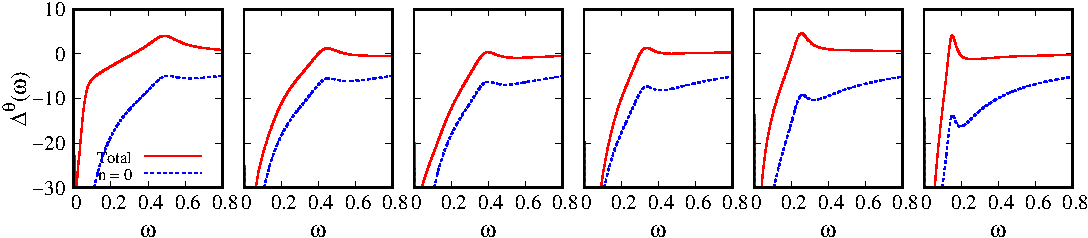
\includegraphics[width=\linewidth]{source_compendium/figures/2605_03277/fig/cld_s0_l2.pdf}
    \caption{CLD. $s=0$, $l=2$, $\theta=43^\circ$.
    The six panels correspond, from left to right, to~$\Lambda=0$, $0.02$, $0.04$, $0.06$, $0.08$, $0.10$.
    The red solid curve denotes the total CLD obtained from the full complex-scaled spectrum.
    The blue dashed curve is the $n=0$ partial reconstruction, in which only the lowest QNM pole is retained in the full-Hamiltonian contribution while the same reference contribution is subtracted.}
    \label{src:2605_03277:fig:cld_s0_l2}
\end{figure}
\begin{figure}[ht]
    \centering
    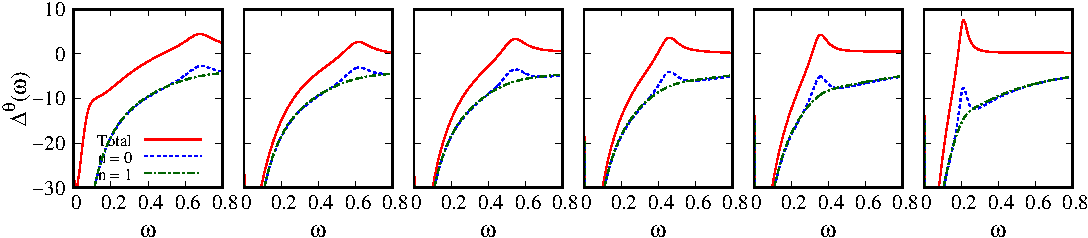
\includegraphics[width=\linewidth]{source_compendium/figures/2605_03277/fig/cld_s0_l3.pdf}
    \caption{CLD. Same as Fig.~\ref{src:2605_03277:fig:cld_s0_l2}, but for $s=0$, $l=3$.
    The green dashed-dotted curve is the $n=1$ partial reconstruction.}
    \label{src:2605_03277:fig:cld_s0_l3}
\end{figure}
\begin{figure}[ht]
    \centering
    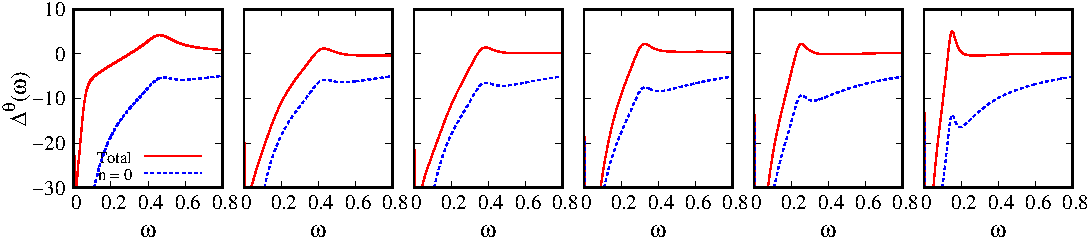
\includegraphics[width=\linewidth]{source_compendium/figures/2605_03277/fig/cld_s1_l2.pdf}
    \caption{CLD. Same as Fig.~\ref{src:2605_03277:fig:cld_s0_l2}, but for $s=1$, $l=2$.}
    \label{src:2605_03277:fig:cld_s1_l2}
\end{figure}
\begin{figure}[ht]
    \centering
    
\includegraphics[width=\linewidth]{source_compendium/figures/2605_03277/fig/cld_s1_l3.pdf}
    \caption{CLD. Same as Fig.~\ref{src:2605_03277:fig:cld_s0_l3}, but for $s=1$, $l=3$.}
    \label{src:2605_03277:fig:cld_s1_l3}
\end{figure}
\begin{figure}[ht]
    \centering
    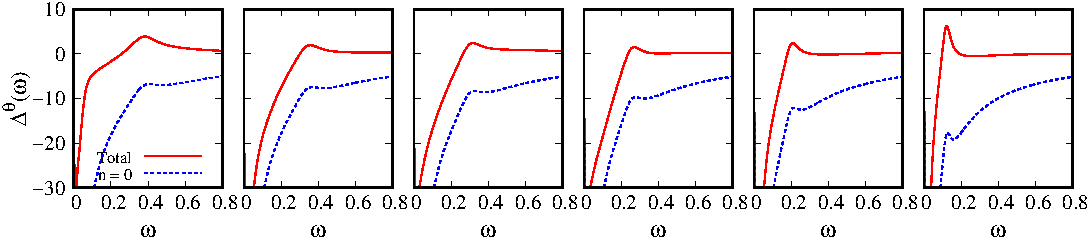
\includegraphics[width=\linewidth]{source_compendium/figures/2605_03277/fig/cld_s2_l2.pdf}
    \caption{CLD. Same as Fig.~\ref{src:2605_03277:fig:cld_s0_l2}, but for $s=2$, $l=2$.}
    \label{src:2605_03277:fig:cld_s2_l2}
\end{figure}
\begin{figure}[ht]
    \centering
    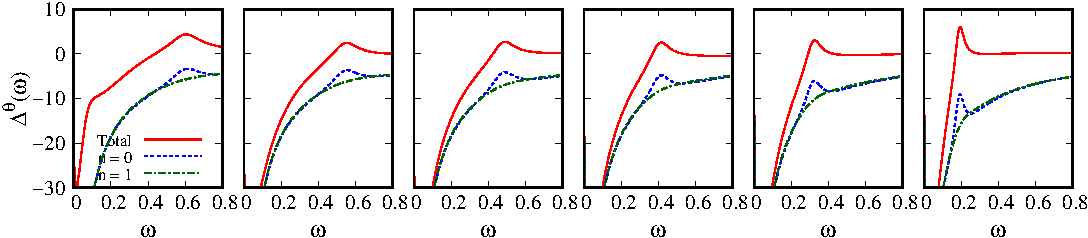
\includegraphics[width=\linewidth]{source_compendium/figures/2605_03277/fig/cld_s2_l3.pdf}
    \caption{CLD. Same as Fig.~\ref{src:2605_03277:fig:cld_s0_l3}, but for $s=2$, $l=3$.}
    \label{src:2605_03277:fig:cld_s2_l3}
\end{figure}
For the representative scalar case with $s=0$ and $l=2$, the total CLD shows
a broad structure for small $\Lambda$.
As $\Lambda$ is increased, the dominant structure moves toward lower
frequency and becomes sharper.
This behavior is consistent with the movement of the lowest QNM frequency
shown in Table~\ref{src:2605_03277:tab:result_ds}: both $\re\omega$ and $|\im\omega|$
decrease as the system approaches the near-Nariai regime.
A smaller value of $|\im\omega|$ corresponds to a narrower resonance
contribution, while the decrease of $\re\omega$ shifts the dominant CLD
structure toward smaller~$\omega$.
The same qualitative behavior is observed for the other spin and angular
momentum sectors.
The detailed peak positions and widths depend on the effective potential,
and hence on $s$ and $l$, but the dominant CLD structure is largely governed
by the lowest QNM pole.
This is seen by comparing the red solid and blue dashed curves: the partial
$n=0$ reconstruction captures the main peak or shoulder structure of the
total CLD, while the remaining poles and nonresonant continuum mainly modify
the smooth background.
The generic near-threshold decrease and the approach to zero at large
$\omega$ are common features of the reference-subtracted continuum response
and should not be attributed to a single resonance alone.
For the $l=3$ cases, the additional $n=1$ partial reconstruction provides
a useful comparison with the first overtone contribution.
Although it gives a visible correction in some frequency regions, the main
peak structure of the total CLD is still primarily governed by the lowest
QNM pole.
This observation is consistent with the behavior found in Appendix~B of our
previous CSM analysis of Schwarzschild and Reissner--Nordström black holes~\cite{Ogawa:2026veu}.
There, the lowest QNM contribution was also found to control the dominant
structure of the CLD, while higher modes and the rotated continuum provided
subleading corrections to the overall background.
The present Schwarzschild--dS results show that the same pole-dominance
pattern persists in the presence of a positive cosmological constant.
\subsection{Discussion}\label{src:2605_03277:sec:discussion}
\subsubsection{On spectral response}
The CLD results clarify how the spectral response of a Schwarzschild--dS
black hole is organized in the CSM representation.
The QNM frequencies listed in Table~\ref{src:2605_03277:tab:result_ds} characterize the
isolated pole sector, whereas the CLD probes the reference-subtracted
continuum response.
The advantage of the CSM is that these two pieces of information are obtained
from the same non-Hermitian spectral problem: isolated QNM poles and the
rotated continuum appear simultaneously in the complex-scaled spectrum.
The comparison between the total CLD and the $n=0$ partial reconstruction
shows that the lowest QNM pole plays a dominant role in shaping the
observable peak structure of the CLD.
This does not mean that the continuum background is negligible.
Rather, the total CLD is produced by the interplay between the pole
contribution and the reference-subtracted continuum.
The lowest QNM pole determines the location and width of the most prominent
structure, while the nonresonant continuum and higher poles contribute to the
smooth background and to the common threshold behavior.
This point is particularly visible in the dependence on the cosmological
constant.
As $\Lambda$ increases, the low-lying QNM frequencies move toward smaller
$\re\omega$ and smaller $|\im\omega|$.
The corresponding CLD peak therefore shifts toward lower frequency and
becomes narrower.
In this sense, the CLD provides a frequency-space representation of the same
spectral reorganization that is seen in the QNM table.
However, unlike the QNM table, the CLD also retains information about the
nonresonant sector.
It is therefore sensitive not only to the position of isolated poles but also
to how the continuum spectrum is redistributed by the black-hole potential.
The behavior near $\omega=0$ should be interpreted with some care.
Both the total CLD and the partial reconstructions exhibit a common
near-threshold decrease and approach zero at sufficiently large $\omega$.
These features are not specific signatures of a single QNM pole.
They arise from the reference-subtracted continuum representation and from
the conversion from the $E$-density to the $\omega$-density in
Eq.~\eqref{src:2605_03277:eq:cld_omega_density}.
For this reason, the most useful information in the present plots is not the
overall sign of the CLD near threshold, but the position, width, and
evolution of the dominant structures as $\Lambda$, $s$, and $l$ are varied.
From this viewpoint, the present results support the following picture.
The ringdown sector is encoded in isolated QNM poles, but the full linear
response is better described as a combined pole-continuum response.
For the low-lying modes considered here, the lowest QNM pole already captures
the leading structure of the CLD.
The remaining continuum contribution provides a nonresonant background that
is invisible in a list of QNM frequencies alone.
Thus, the CLD complements the usual QNM analysis by giving a direct diagnostic
of how the continuum sector participates in the black-hole spectral response.
\subsubsection{CLD, transmission phase, and greybody factors}
\label{src:2605_03277:sec:discussion-greybody}
It is useful to clarify the relation between the present CLD analysis and
greybody factors.
Greybody factors are transmission probabilities associated with black-hole
scattering problems.
They describe how the effective potential outside the black hole modifies the
spectrum of radiation from a perfect blackbody spectrum and are therefore
more directly connected to observable fluxes.
They have been studied in a variety of black-hole backgrounds, including
higher-dimensional, charged, dS, and AdS cases~\cite{Harmark:2007jy}.
More recently, greybody factors have also been discussed in connection with
black-hole ringdown amplitudes and as quantities complementary to the usual
QNM description~\cite{Oshita:2023cjz,Konoplya:2024lir}.
The CLD is not itself a transmission coefficient.
Rather, it measures the change of the continuum density of states relative to
a reference problem.
In the CSM, the CLD~\eqref{eq:cld-csm} is evaluated as
\begin{align}
    \Delta \rho^\theta(E)
    &=
    -\frac{1}{\pi}
    \im
    \Tr
    \left[
        \frac{1}{E-H^\theta}
        -
        \frac{1}{E-H_0^\theta}
    \right]
    \notag\\
    &=
    -\frac{1}{\pi}
    \im
    \left[
        \sum_\nu \frac{1}{E-E^\theta_\nu}
        -
        \sum_{\nu'} \frac{1}{E-E^\theta_{0,\nu'}}
    \right],
    \label{src:2605_03277:eq:cld_csm_nu}
\end{align}
where $H^\theta$ and $H_0^\theta$ are the complex-scaled full and reference
Hamiltonians, respectively, and
$E^\theta_\nu$ and $E^\theta_{0,\nu'}$ denote their complex eigenvalues.
Equation~\eqref{src:2605_03277:eq:cld_csm_nu} naturally decomposes the CLD into individual
spectral contributions,
\begin{align}
    \Delta\rho^\theta(E)
    =
    \sum_\nu \rho^\theta_\nu(E)
    -
    \sum_{\nu'} \rho^\theta_{0,\nu'}(E).
\end{align}
This decomposition is one of the practical advantages of the CSM:
resonance poles and the rotated continuum can be analyzed within the same
non-Hermitian spectral representation.
In ordinary one-dimensional scattering theory, the change in the density of
states is related to the energy derivative of the phase of the transmission
amplitude~\cite{Avishai:1985}.
Writing
\begin{align}
    t(E)=|t(E)|\rme^{\rmi \delta(E)},
\end{align}
one obtains, up to the conventional normalization of the phase,
\begin{align}
    \Delta\rho(E)
    =
    \frac{1}{\pi}
    \frac{\rmd \delta(E)}{\rmd E}.
    \label{src:2605_03277:eq:cld_phase_relation}
\end{align}
Equivalently,
\begin{align}
    \delta(E)
    =
    \pi
    \int^E \rmd E'\,\Delta\rho(E')
    +
    \delta_0 ,
    \label{src:2605_03277:eq:phase_from_cld}
\end{align}
where $\delta_0$ is an energy-independent constant fixed by the choice of
reference phase.
Using the CSM decomposition of Eq.~\eqref{src:2605_03277:eq:cld_csm_nu}, this phase may be
written as
\begin{align}
    \delta(E)
    =
    \sum_\nu \delta_\nu(E)
    -
    \sum_{\nu'} \delta_{0,\nu'}(E)
    +
    \delta_0 ,
\end{align}
with
\begin{align}
    \delta_\nu(E)
    =
    \pi\int^E \rmd E'\,\rho^\theta_\nu(E').
\end{align}
Thus, the CSM gives a way of separating the transmission phase into
contributions from resonance and continuum eigenstates.
This observation suggests a possible bridge to greybody factors.
For a black-hole scattering problem, the greybody factor is essentially a
transmission probability,
\begin{align}
    \Gamma(E)=|t(E)|^2 ,
\end{align}
up to possible channel-dependent normalization factors.
The CLD does not by itself determine $\Gamma(E)$, because
Eq.~\eqref{src:2605_03277:eq:cld_phase_relation} gives the phase of the transmission
amplitude rather than its modulus.
Nevertheless, the two quantities probe different aspects of the same
underlying scattering problem:
the greybody factor probes the probability for transmission through the
black-hole effective potential, whereas the CLD probes the rearrangement of
the continuum spectrum.
From the present CSM viewpoint, the most promising role of the CLD is not to
replace a direct real-frequency scattering calculation of the greybody factor.
Rather, the CSM can decompose the spectral phase response into resonant and
nonresonant parts.
If the transmission amplitude is written as
\begin{align}
    t(E)
    =
    |t(E)|
    \rme^{\rmi \delta(E)},
\end{align}
then the CSM decomposition gives, at least formally,
\begin{align}
    t(E)
    =
    |t(E)|
    \prod_\nu \rme^{\rmi \delta_\nu(E)}
    \prod_{\nu'} \rme^{-\rmi \delta_{0,\nu'}(E)}
    \times \rme^{\rmi \delta_0}.
    \label{src:2605_03277:eq:t_phase_decomposition}
\end{align}
This expression should be understood as a decomposition of the phase part of
the transmission amplitude, not of the transmission probability itself.
A direct computation of greybody factors requires the modulus $|t(E)|$, which
is most directly obtained from a real-frequency scattering calculation with
appropriate boundary conditions.
However, Eq.~\eqref{src:2605_03277:eq:t_phase_decomposition} indicates what the CSM can add:
it can identify how much of the scattering phase, and hence of the continuum
spectral response, is controlled by QNM poles and how much is carried by the
nonresonant background.
In this sense, the CLD provides a bridge between the pole-based QNM
description and more directly observable scattering quantities such as
greybody factors.
A full CSM-based reconstruction of greybody factors, including both phase and
modulus information, is left for future work.
\subsection{Further applications}\label{src:2605_03277:sec:application}
\enlargethispage{4pt}
\subsubsection{Coupled-channel systems: toward stringy black holes}
Recent work on the two-dimensional Mandal--Sengupta--Wadia (MSW) black hole shows that intrinsic
metric--dilaton perturbations can be reduced not to a single Schr\"odinger
equation but to a coupled matrix Schr\"odinger problem,
\begin{align}
    -\frac{\rmd^2}{\rmd r_*^2}\Phi(r_*)
    +
    \vsub{V}{eff}(r_*)\Phi(r_*)
    =
    \omega^2 \Phi(r_*),
    \label{src:2605_03277:eq:string_coupled_eq}
\end{align}
with a $2\times2$ effective potential matrix.
% Here, $\Phi$ has two degrees of freedom from the metric perturbation~$\psi$ and the dilaton one $\chi$ as
% \begin{align}
%     \begin{pmatrix}
%         \phi_0 \chi \\ \psi
%     \end{pmatrix} =
%     \begin{pmatrix}
%         1 & 0 \\ \phi_0^{-2} & 1
%     \end{pmatrix}
%     \Phi ,
%     \qquad
%     \phi_0 = \sqrt{\frac{r}{M}}
%     = \sqrt{1 + \frac{1}{M\Lambda} \rme^{2\Lambda r_*} } ,
% \end{align}
Here, $\Phi$ is a two-component field describing the coupled
metric--dilaton perturbation sector.
In the field basis used in Ref.~\cite{Bian:2026crb},\footnote{%
This basis is obtained by redefining the original metric and dilaton
perturbations so that Eq.~\eqref{src:2605_03277:eq:string_coupled_eq} has a
Schr\"odinger-type form without first-derivative terms.}
the elements of the effective potential are given by
\begin{align}
    \vsub{V}{eff}^{11,22}
    &= \frac{8\Lambda^2 \rme^{2\Lambda r_*}}{M\Lambda + \rme^{2\Lambda r_*}} ,
    \\
    \vsub{V}{eff}^{12}
    &= \frac{4\vsub{V}{eff}^{11}}{8-\vsub{V}{eff}^{11}/\Lambda^2} ,
    \\
    \vsub{V}{eff}^{21}
    &= \frac{1}{128} \vsub{V}{eff}^{11}
    \left(8-\frac{\vsub{V}{eff}^{11}}{\Lambda^2}\right)
    \left(32-\frac{\vsub{V}{eff}^{11}}{\Lambda^2}\right).
    \label{src:2605_03277:eq:string_pot}
\end{align}
Usually, the kinetic term and the overlap matrix can be evaluated
analytically for the basis functions used in the numerical variational method,
whereas the potential matrix elements require numerical integration.
Here, let us adopt the Polynomial $\times$ real range Gaussian basis.
Using Kummer's transformation for the confluent hypergeometric function, we
obtain
\begin{align}
    \int_{-\infty}^\infty \rmd r_*\, r_*^n \rme^{-\alpha r_*^2} \vsub{V}{eff}^{12}
   %  \notag\\
   %  &= 
   %  \frac{2 \Lambda  \alpha ^{-\frac{n}{2}-1} \left(\sqrt{\alpha } \left((-1)^n+1\right)
   % \Gamma \left(\frac{n+1}{2}\right) \,
   % _1F_1\left(\frac{n+1}{2};\frac{1}{2};\frac{\Lambda ^2}{\alpha }\right)-\lambda 
   % \left((-1)^n-1\right) n \Gamma \left(\frac{n}{2}\right) \,
   % _1F_1\left(\frac{n}{2}+1;\frac{3}{2};\frac{\Lambda ^2}{\alpha
   % }\right)\right)}{M}
   % \\
   &= 
\begin{cases}
\frac{
4\sqrt{\pi}\,k!\,\Lambda
}{
M
}
\alpha^{-k-\frac{1}{2}}
\rme^{\frac{\Lambda^2}{\alpha}}
L_k^{-\frac{1}{2}}
\!\left(
-\frac{\Lambda^2}{\alpha}
\right) & \text{for $n=2k$} ,
\\
\frac{
4\sqrt{\pi}\,k!\,\Lambda^2
}{
M
}
\alpha^{-k-\frac{3}{2}}
\rme^{\frac{\Lambda^2}{\alpha}}
L_k^{\frac{1}{2}}
\!\left(
-\frac{\Lambda^2}{\alpha}
\right) & \text{for $n=2k+1$} .
\end{cases}
  \label{src:2605_03277:eq:kummer_transf}
\end{align}
Here, $L_k^a(z)$ denotes the generalized Laguerre polynomial.
Thus, the potential matrix element associated with $\vsub{V}{eff}^{12}$ can
be evaluated analytically, without performing the numerical integration.\footnote{%
In the coupled-channel problem, some off-diagonal components of the effective
potential can become exponentially large in the original field basis, while
the eigenvalues of the potential matrix remain finite.
This indicates that the difficulty is not a physical divergence of the
potential, but a numerical conditioning problem associated with the choice of
channel basis.
A suitable channel rescaling or matrix balancing is therefore required before
performing the complex-scaled diagonalization. See Sec.~\ref{src:2605_03277:sec:balance}.}
We next apply the CSM to the coupled-channel system
\eqref{src:2605_03277:eq:string_coupled_eq}.
A characteristic feature of this problem is that the asymptotic effective
potential has two eigenvalue thresholds.
Consequently, the complex-scaled spectrum contains two rotated continuum
branches, each starting from a different threshold.
This is in contrast to the single-channel Schwarzschild--dS examples
discussed above, where the continuum branch starts from a single threshold.
The result is shown in Fig.~\ref{src:2605_03277:fig:stringy_coupled_spectrum}.
The two lines show the corresponding complex-scaled continua
rotated by the angle $2\theta$.
\begin{figure}[htbp]
    \centering
    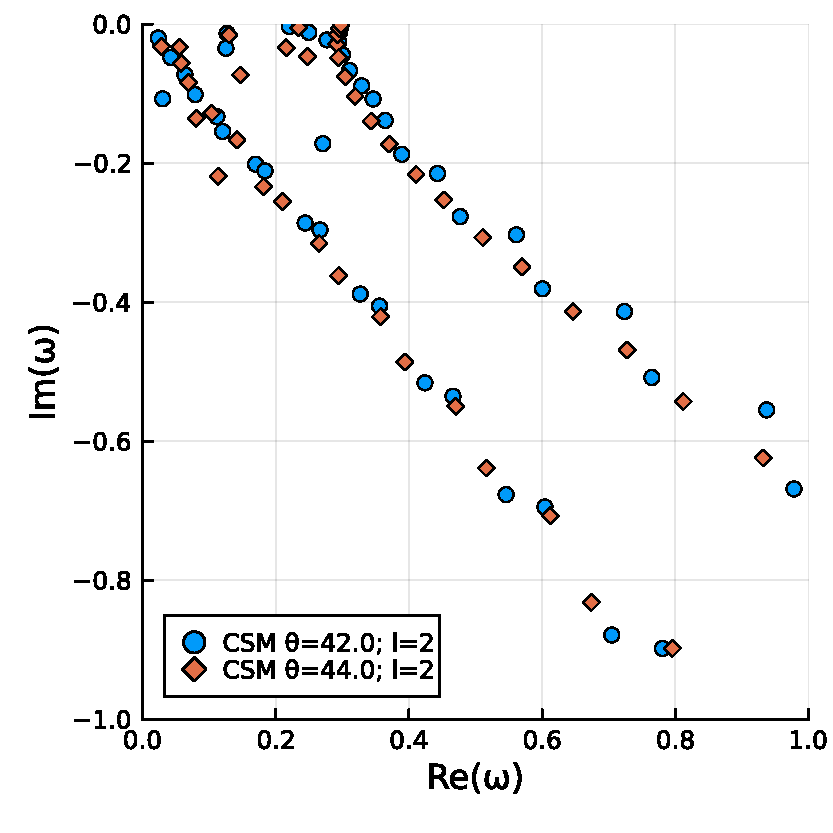
\includegraphics[width=0.75\columnwidth]{source_compendium/figures/2605_03277/fig/stringy_coupled_spectrum.pdf}
    \caption{Complex-scaled spectrum for the coupled-channel MSW black-hole
    perturbation problem with $\Lambda=0.08$. $l=2$.
    The scaling angle is $\theta=42^\circ$ and $44^\circ$.
    We set $i_{\max}=50$, $r_0=0.1$, and $r_{*\max}=80$.
    %  $x_{\max}=500$, $x_{\min}=-500$.
    Because the asymptotic effective potential has two eigenvalue thresholds,
    two continuum branches are observed.
    Within the parameter sets examined in this work, no stable isolated
    resonance eigenvalue was identified for $\theta<45^\circ$.
    }
    \label{src:2605_03277:fig:stringy_coupled_spectrum}
\end{figure}
To examine whether an isolated QNM eigenvalue can be exposed between the real
axis and the rotated continua, we performed a parameter scan over the basis
size, Gaussian range, integration range, and scaling angle.
The representative parameter sets used in this search are summarized in
Table~\ref{src:2605_03277:tab:stringy_parameter_sets}.
In all cases, we restricted the scaling angle to
\begin{align}
    \theta < \frac{\pi}{4},
\end{align}
which is the practical range of the present real-range Gaussian basis.
\begin{table}[htbp]
\centering
\caption{Representative parameter sets used in the CSM search for isolated resonance
eigenvalues in the coupled-channel MSW black-hole perturbation problem.
}
\label{src:2605_03277:tab:stringy_parameter_sets}
\begin{tabular}{ccccccc}
\toprule
Set & $i_{\max}$ & $p_{\max}$ & $r_{*0}$ & $r_{*\max}$ & $\theta$ & $\Lambda$ \\
\midrule
1 & 40 & 3 & 0.1 & 60 & $30^\circ$--$44^\circ$ & $0.01$--$0.1$ \\
2 & 40 & 3 & 0.1 & 80 & $30^\circ$--$44^\circ$ & $0.01$--$0.1$ \\
3 & 50 & 3 & 0.1 & 60 & $30^\circ$--$44^\circ$ & $0.01$--$0.1$ \\
4 & 50 & 3 & 0.1 & 80 & $30^\circ$--$44^\circ$ & $0.01$--$0.1$ \\
\bottomrule
\end{tabular}
\end{table}
Within this survey, we did not find a stable isolated eigenvalue that can be
identified as a QNM for $\theta<45^\circ$.
This should not be interpreted as evidence for the absence of QNMs in the
underlying stringy black-hole perturbation problem.
Rather, it indicates a limitation of the present real-range Gaussian CSM
implementation.
Indeed, the QNMs reported in Ref.~\cite{Bian:2026crb} are strongly damped in
the parameter region studied there.
For such modes, the corresponding position in the complex
$E=\omega^2$ plane can lie in a region that requires a larger rotation angle
to expose the pole from the continuum background.
However, the present basis representation becomes ill-conditioned as
$\theta$ approaches $\pi/4$, and therefore does not allow us to reliably
search for such poles beyond this angle.
The present result is nevertheless informative.
It shows that the coupled-channel CSM calculation correctly resolves the
multi-threshold continuum structure, while also revealing that the extraction
of highly damped QNM poles requires further stabilization.
Possible improvements include complex-range Gaussian bases, exterior complex
scaling, and channel-basis or matrix balancing of the type discussed in
Sec.~\ref{src:2605_03277:sec:balance}.
We therefore regard the stringy coupled-channel example as a useful
diagnostic problem for future extensions of the CSM framework, rather than as
a completed QNM computation in the present implementation.
\subsubsection{Higher-dimensional dS black holes}
As another natural direction, one may consider higher-dimensional
Schwarzschild--dS spacetimes.
In $d$ dimensions, the metric may be written as~\cite{Kodama:2003jz,Ishibashi:2003ap,Ishibashi:2011ws}\footnote{%
The black-hole mass parameter $M$ is
related to a horizon radius $r_0$ as
\begin{align}
    M = \frac{(d-2)A_{d-2}r_0^{d-3}}{16\pi G_d},
    \qquad
    A_{d-2} = \frac{2\pi^{(d-1)/2}}{\Gamma((d-1)/2)} ,
\end{align}
where $A_{d-2}$ denotes the area of the unit $(d-2)$-sphere.}
\begin{align}
    \rmd s^2 &= -f_d(r) \rmd t^2+f_d^{-1}(r)\rmd r^2+r^2 \rmd\Omega_{d-2},
    \label{src:2605_03277:eq:ds_d_metric}
    \\
    f_d(r) &= K-\lambda r^2-\frac{2M}{r^{d-3}},
    \label{src:2605_03277:eq:ds_d_metric_fn}
    \\
    \lambda &\equiv \frac{2\Lambda}{(d-1)(d-2)}.
\end{align}
$K$ denotes the sectional curvature of the $(d-2)$-dimensional base space.
In the present discussion, we mainly restrict ourselves to the case $K=1$.
For tensor-type perturbations on the $(d-2)$-dimensional angular sector with~$d\geq5$, the
effective potential is given by
\begin{align}
    V_T(r)
    &=
    \frac{f_d(r)}{r^2}
    \left[
        l(l+d-3)
        +\frac{(d-2)r f'_d(r)}{2}
        +\frac{(d-2)(d-4)f_d(r)}{4}
    \right].
    \label{src:2605_03277:eq:ds_d_pot_tensor}
\end{align}
For vector-type perturbations, one has
\begin{align}
    V_V(r)
    &=
    \frac{f_d(r)}{r^2}
    \left[
        l(l+d-3)
        +(d-4)
        +\frac{d(d-2)f_d(r)}{4}
        -\frac{(d-2)r f'_d(r)}{2}
    \right].
    \label{src:2605_03277:eq:ds_d_pot_vec}
\end{align}
The scalar-type potential is considerably more complicated.
These expressions suggest that higher-dimensional dS black holes provide
a natural class of backgrounds in which the present CSM framework may be
extended.
At least for the tensor- and vector-type sectors, the perturbation equations
remain of Schr\"odinger type, so that the basic spectral strategy should carry
over in a relatively direct manner.
As a simple illustration of the higher-dimensional extension, we also perform
a trial calculation for five-dimensional Schwarzschild--dS (Schwarzschild--dS$_5$) black holes.
Here we do not attempt a systematic survey of the higher-dimensional
parameter space.
Rather, our purpose is to check whether the same CSM prescription used in the
four-dimensional analysis can be applied directly to the tensor- and
vector-type master equations.
Figure~\ref{src:2605_03277:fig:qnm_ds_d_s2} shows the result for the Schwarzschild--dS$_5$
case in the tensor-type sector.
The complex-scaled spectra are shown for two angular momenta, $l=2$ and
$l=3$, and for two scaling angles, $\theta=40^\circ$ and $42^\circ$.
As in the four-dimensional case, the complex-scaled continuum is rotated in
the complex energy plane, and resonance candidates are identified as isolated
eigenvalues that are separated from the rotated continuum and remain stable
under a moderate change of the scaling angle.
\begin{figure}[ht]
    \centering
    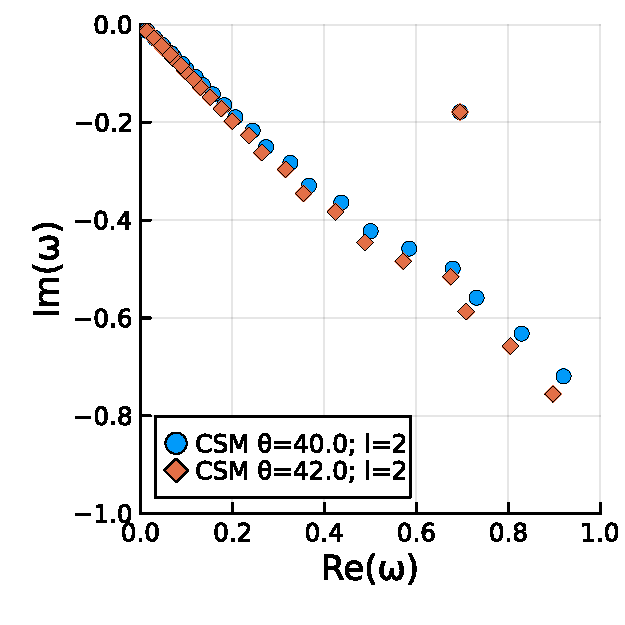
\includegraphics[width=0.45\columnwidth]{source_compendium/figures/2605_03277/fig/ene_ds_d_s2_l2.pdf}
    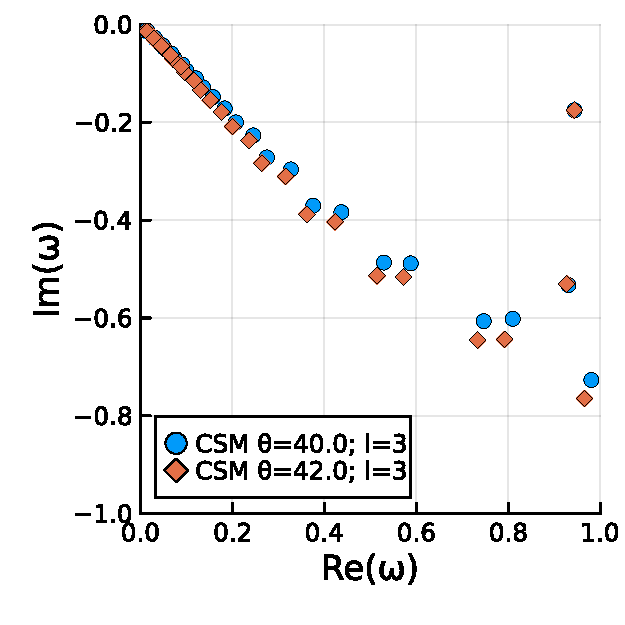
\includegraphics[width=0.45\columnwidth]{source_compendium/figures/2605_03277/fig/ene_ds_d_s2_l3.pdf}
    \caption{The Schwarzschild--dS$_5$ case for the tensor-type sector.
    $\Lambda=0.4$.
    The scaling angle is taken to be~$\theta=40^\circ$, $42^\circ$.
    We take  $i_{\max}=30$, $r_{*0}=0.1$, and $r_{*\max}=60$.
    $l=2$ on the left panel and $l=3$ on the right panel.}
    \label{src:2605_03277:fig:qnm_ds_d_s2}
\end{figure}
Figure~\ref{src:2605_03277:fig:qnm_ds_d_s1} shows the corresponding example for the
Schwarzschild--dS$_5$ case in the vector-type sector.
Again, the same qualitative spectral structure is observed.
The appearance of stable isolated eigenvalues in these trial calculations
suggests that the CSM strategy can be extended to higher-dimensional
Schwarzschild--dS backgrounds at least for the tensor- and vector-type
sectors.
The present numerical results are in good agreement with those reported
by Konoplya~\cite{Konoplya:2003dd}.\footnote{%
When comparing the numerical values, we take into account the difference in
the normalization of the cosmological-constant parameter.  The cosmological
constant in the present convention is related to that used in
Ref.~\cite{Konoplya:2003dd} by~$\Lambda=2\vsub{\Lambda}{Konoplya}.$}
A detailed convergence analysis and a systematic comparison among different
dimensions, angular momenta, and perturbation sectors are left for future
work.
\begin{figure}[ht]
    \centering
    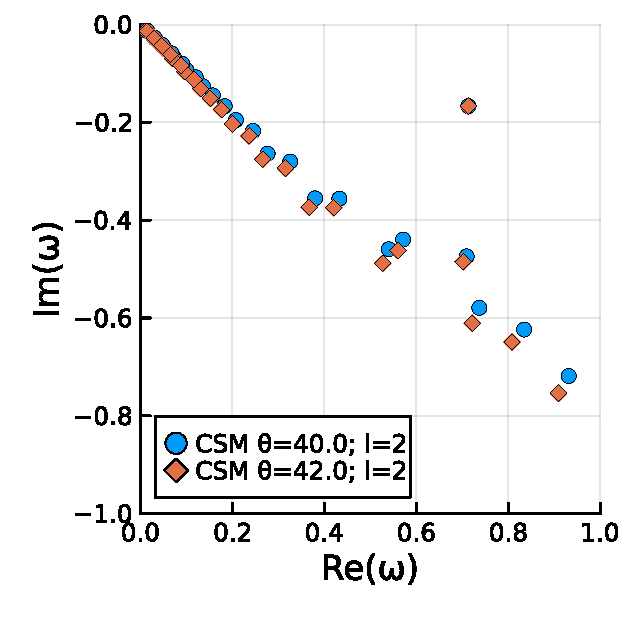
\includegraphics[width=0.45\columnwidth]{source_compendium/figures/2605_03277/fig/ene_ds_d_s1_l2.pdf}
    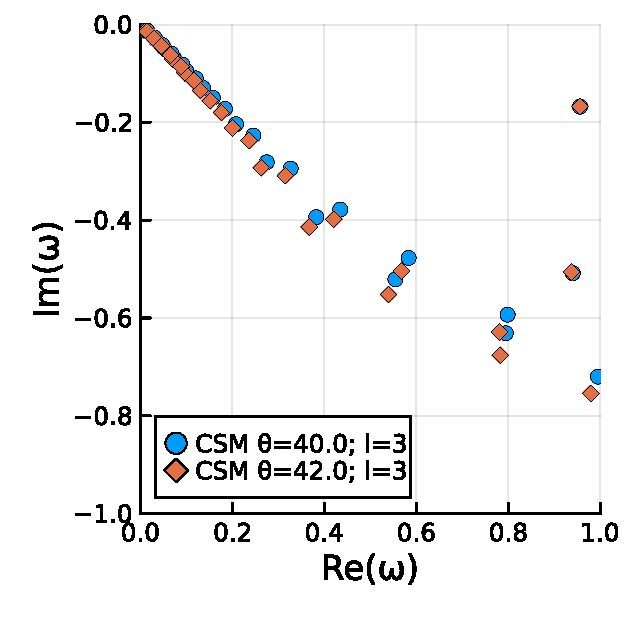
\includegraphics[width=0.45\columnwidth]{source_compendium/figures/2605_03277/fig/ene_ds_d_s1_l3.pdf}
    \caption{The Schwarzschild--dS$_5$ case for the vector-type sector.
    $\Lambda=0.4$.
    The scaling angle is taken to be~$\theta=40^\circ$, $42^\circ$.
    We take  $i_{\max}=30$, $r_{*0}=0.1$, and $r_{*\max}=60$.
    $l=2$ on the left panel and $l=3$ on the right panel.}
    \label{src:2605_03277:fig:qnm_ds_d_s1}
\end{figure}
\subsection{Exponentially growing matrix blocks in diagonalization}\label{src:2605_03277:sec:balance}
Let us consider the generalized complex eigenvalue problem
\begin{align}
    H c = E N c ,
    \label{src:2605_03277:eq:generalized-evp-gaussian}
\end{align}
or, equivalently,
\begin{align}
    \sum_j
    \left[
        H_{ij}-E N_{ij}
    \right] c_j
    =0 .
\end{align}
For a two-channel problem, the Hamiltonian matrix has the block structure
\begin{align}
    H
    =
    \begin{pmatrix}
        T_{11}+V_{11} & V_{12} \\
        V_{21}        & T_{22}+V_{22}
    \end{pmatrix}.
\end{align}
In coupled-channel problems such as string-inspired black-hole perturbations,
some off-diagonal blocks can become exponentially large in the original field
basis.
For example, as seen in Eq.~\eqref{src:2605_03277:eq:kummer_transf}, the matrix element
associated with $V_{12}$ contains the factor
\begin{align}
    \rme^{\frac{\Lambda^2}{\alpha}},
\end{align}
which can become very large for small Gaussian range parameters~$\alpha$.
This does not necessarily indicate a physical divergence of the effective
potential.
Rather, it can reflect a poor conditioning of the chosen channel basis.
In such a situation, the direct diagonalization of Eq.~\eqref{src:2605_03277:eq:generalized-evp-gaussian}
becomes numerically unstable.
\subsubsection{Block balancing}
A simple stabilization strategy is to apply a similarity transformation at the
matrix level.
We introduce the block scaling matrix
\begin{align}
    S
    =
    \begin{pmatrix}
        I & 0 \\
        0 & s I
    \end{pmatrix},
    \qquad
    s>0 ,
\end{align}
and write
\begin{align}
    c = S \tilde{c}.
\end{align}
Then Eq.~\eqref{src:2605_03277:eq:generalized-evp-gaussian} becomes
\begin{align}
    \left(
        S^{-1} H S
        -
        E S^{-1} N S
    \right)
    \tilde{c}
    =
    0 .
\end{align}
The scaled Hamiltonian is
\begin{align}
    S^{-1} H S
    =
    \begin{pmatrix}
        T_{11}+V_{11} & s V_{12} \\
        s^{-1}V_{21} & T_{22}+V_{22}
    \end{pmatrix}.
\end{align}
The eigenvalues are unchanged by this similarity transformation, while the
conditioning of the matrix problem can be improved.
A natural choice is to balance the norms of the two off-diagonal blocks:
\begin{align}
    s
    =
    \sqrt{
        \frac{
            \lVert V_{21}\rVert
        }{
            \lVert V_{12}\rVert
        }
    } .
\end{align}
Alternatively, if the exponential growth is dominated by the factor
$\rme^{\Lambda^2/\alpha}$, one may use a scale estimate such as
\begin{align}
    s
    \sim
    \rme^{
        -\frac{\Lambda^2}{\vsub{\alpha}{eff}}
    },
\end{align}
where $\vsub{\alpha}{eff}$ is a representative Gaussian range parameter.
The norm-balancing prescription is usually more robust, because it uses the
actual matrix elements after discretization.
\subsubsection{Channel-basis balancing}
A more structural approach is to change the channel basis before
discretization.
Consider the coupled Schr\"odinger-type equation
\begin{align}
    -
    \frac{\rmd^2}{\rmd r_*^2}
    \Phi(r_*)
    +
    V(r_*)\Phi(r_*)
    =
    E\Phi(r_*) .
\end{align}
We introduce a local channel rescaling
\begin{align}
    \Phi(r_*)
    =
    D(r_*)\Xi(r_*),
    \qquad
    D(r_*)
    =
    \begin{pmatrix}
        \rme^{\Lambda r_*} & 0 \\
        0               & \rme^{-\Lambda r_*}
    \end{pmatrix}.
\end{align}
Substituting this into the original equation and multiplying by $D^{-1}$ from
the left, we obtain
\begin{align}
    -
    \frac{\rmd^2}{\rmd r_*^2}
    \Xi
    -
    2D^{-1}D'
    \frac{\rmd}{\rmd r_*}
    \Xi
    +
    \left(
        D^{-1}VD
        -
        D^{-1}D''
    \right)
    \Xi
    =
    E\Xi .
    \label{src:2605_03277:eq:channel-balanced-eq}
\end{align}
Thus, the exponentially unbalanced off-diagonal potential is replaced by
\begin{align}
    V_{12}
    \mapsto
    \rme^{-2\Lambda r_*} V_{12},
    \qquad
    V_{21}
    \mapsto
    \rme^{2\Lambda r_*} V_{21}.
\end{align}
This can reduce the exponential hierarchy between the two off-diagonal
blocks.
The price of this transformation is the appearance of a first-derivative
coupling term,
\begin{align}
    -2D^{-1}D'
    \frac{\rmd}{\rmd r_*}\Xi .
\end{align}
Therefore, the resulting problem is no longer in the standard
Schr\"odinger form without first derivatives.
Nevertheless, this formulation may be numerically preferable if the original
off-diagonal blocks are so unbalanced that the direct diagonalization becomes
ill-conditioned.
In practice, the matrix-level block balancing is the simplest first test,
because it does not modify the differential equation.
If the instability persists, the channel-basis balancing of
Eq.~\eqref{src:2605_03277:eq:channel-balanced-eq} provides a more systematic way to remove
the exponential hierarchy at the level of the continuum problem.

\subsection*{Laboratory checkpoint}
Before moving to the next stage, perform the following checks without copying
the displayed final answer.
\begin{enumerate}
  \item Derive the local ingoing/outgoing exponents at both horizons and translate them into admissible complex-deformation wedges.
  \item Reproduce one de Sitter QNM spectrum together with its continuum level density while varying the cosmological parameter.
  \item For a coupled example, monitor the norms of every matrix block and demonstrate the effect of block balancing on the stable poles.
\end{enumerate}
